% !TeX program = lualatex

% setup
\documentclass[
hyperref={bookmarks=false},
xcolor={dvipsnames,svgnames*,x11names*}, 
12pt
]{beamer}
\usepackage{../beamertheme/beamerinnerthemetb}
\usepackage{../beamertheme/beamerouterthemetb}
\usepackage{../beamertheme/beamercolorthemetb}
\usepackage{../beamertheme/beamerthemetb}

% packages
\usepackage{emoji}
\usepackage{graphicx}
\usepackage{xurl}
\usepackage{epigraph}
\setlength\epigraphwidth{\linewidth}

% options
\setlength{\leftmargini}{0.08cm}
\hypersetup{
	pdfauthor={Andrea Gilardi},
	colorlinks=true,
	urlcolor=Blue
}

% metadata
\title{R4DS - Unit 2: Debugging}
\author{Andrea Gilardi}
\date{\today}

\begin{document}
\inserttitlepage

\begin{frame}{Outline and main concepts}
\vspace{-0.5cm}
\begin{itemize}
\itemsep 3ex
\item The objective of this unit is to learn the basic tools for debugging R code using R and Rstudio. 
\item We will start with a little of theory and then I will introduce the most common approaches with a series of example. 
\item At the end, we will just briefly recall the main venues that can be consulted when asking for help and the best practices required to interact with those systems.
\end{itemize}
\end{frame}

\begin{frame}{But first...}
\vspace{-0.5cm}
\begin{itemize}
\itemsep 2ex
\item Let's start with a quote by \href{https://heather.cs.ucdavis.edu/matloff.html}{Norm Matloff}: \emph{``Finding your bug is a process of confirming the many things that you believe are true — until you find one which is not true"}\dots
\item which let me introduce our \textbf{best} programming companion: \href{https://en.wikipedia.org/wiki/Rubber_duck_debugging}{the debugging duck}!
\end{itemize}
\begin{figure}
\centering
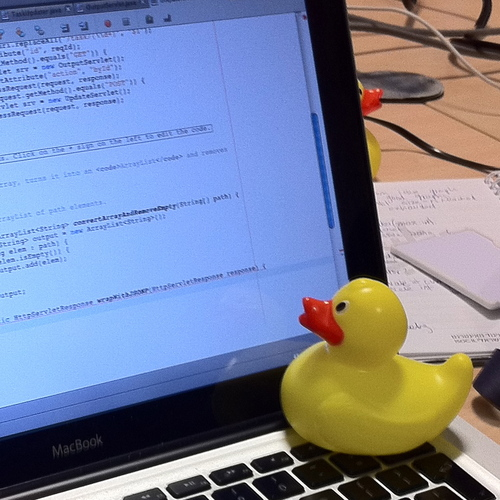
\includegraphics[width=0.36\linewidth]{figures/rubber-duck-assisting-with-debugging}
\end{figure}
\end{frame}

\begin{frame}{Rubber Duck Debugging}
\vspace{-0.5cm}
{\small
\begin{enumerate}
\item Beg, borrow, steal, buy, fabricate or otherwise obtain a rubber duck (bathtub variety).
\item Place rubber duck on desk and inform it you are just going to go over some code with it, if that’s all right.
\item Explain to the duck what your code is supposed to do, and then go into detail and explain your code line by line.
\item At some point you will tell the duck what you are doing next and then realise that that is not in fact what you are actually doing. The duck will sit there serenely, happy in the knowledge that it has helped you on your way.
\end{enumerate}
}

\textbf{Note:} A \href{https://sites.google.com/unimib.it/camerlenghi-federico/}{\textbf{``coworker"}} might be able to substitute for the duck\dots
\end{frame}

\begin{frame}{Just to be a little more concrete...}
\vspace{-0.5cm}
Now we are going to review the following functions: 
\begin{itemize}
\itemsep 3ex
\item \texttt{traceback():} Inspect the call stack;
\item \texttt{browser():} Manually enter into debug state;
\item \texttt{debug(): } Set the debug state for any function;
\item \texttt{try() + tryCatch(): } Condition handling! 
\end{itemize}
\end{frame}

\begin{frame}{And if I cannot debug my code? }
\vspace{-0.5cm}
\begin{itemize}
\itemsep 2ex
\item You need to ask for help! \textit{But where?} \emoji{loudly-crying-face}
\item Google your problem! Maybe you are lucky,  \href{https://imgs.xkcd.com/comics/wisdom_of_the_ancients.png}{usually no}... 
\item If you face a problem with a function in a contributed package, you should contact its maintainer and, whenever possible, raise an issue in the corresponding github repo. 
\item If you have a generic programming question, you can ask it in several forums (e.g. \href{https://stackoverflow.com/questions/tagged/r}{SO}) or \href{https://www.r-project.org/mail.html}{mailing lists}.
\item In any case, please remember that the people maintaining the software and the package are volunteers and you should present your problem in the best possible format (see also \texttt{fortunes::fortune(107)} and \href{https://stackoverflow.com/questions/5963269/how-to-make-a-great-r-reproducible-example}{this} SO thread). 
\end{itemize}
\end{frame}

\begin{frame}{\texttt{reprex::reprex()}}
\vspace{-0.5cm}
\begin{figure}
\centering

\includegraphics[width=\linewidth]{figures/reprex.png}
\end{figure}
\textbf{Source: } \url{https://reprex.tidyverse.org/}.
\end{frame}

% To receive useful feedback, please provide the complete context of the problem, including a reprex. The purpose of a reprex, or reproducible example1, is to eliminate the knowledge gaps, misunderstandings, and hidden assumptions where bugs hide. A reprex is a sample of complete, self-contained, runnable code that fully emulates and reproduces the problem. The code should look clean and readable, be as short and concise as possible, run in as few seconds as possible, and contain only the details most relevant to troubleshooting. You can embed the code inline in your question, or you can upload it to a public repository and post the link. Regardless, please expect that anyone trying to help will read all the code and run the enclosed _targets.R file on their own private computer. Please make this utterly empirical process as quick and easy as possible for the people who volunteer their valuable time and energy to answer questions.

\end{document}
